\chapter{Decidability Problem With Logic Engines}
\begin{figure}[!htbp]
\begin{center}
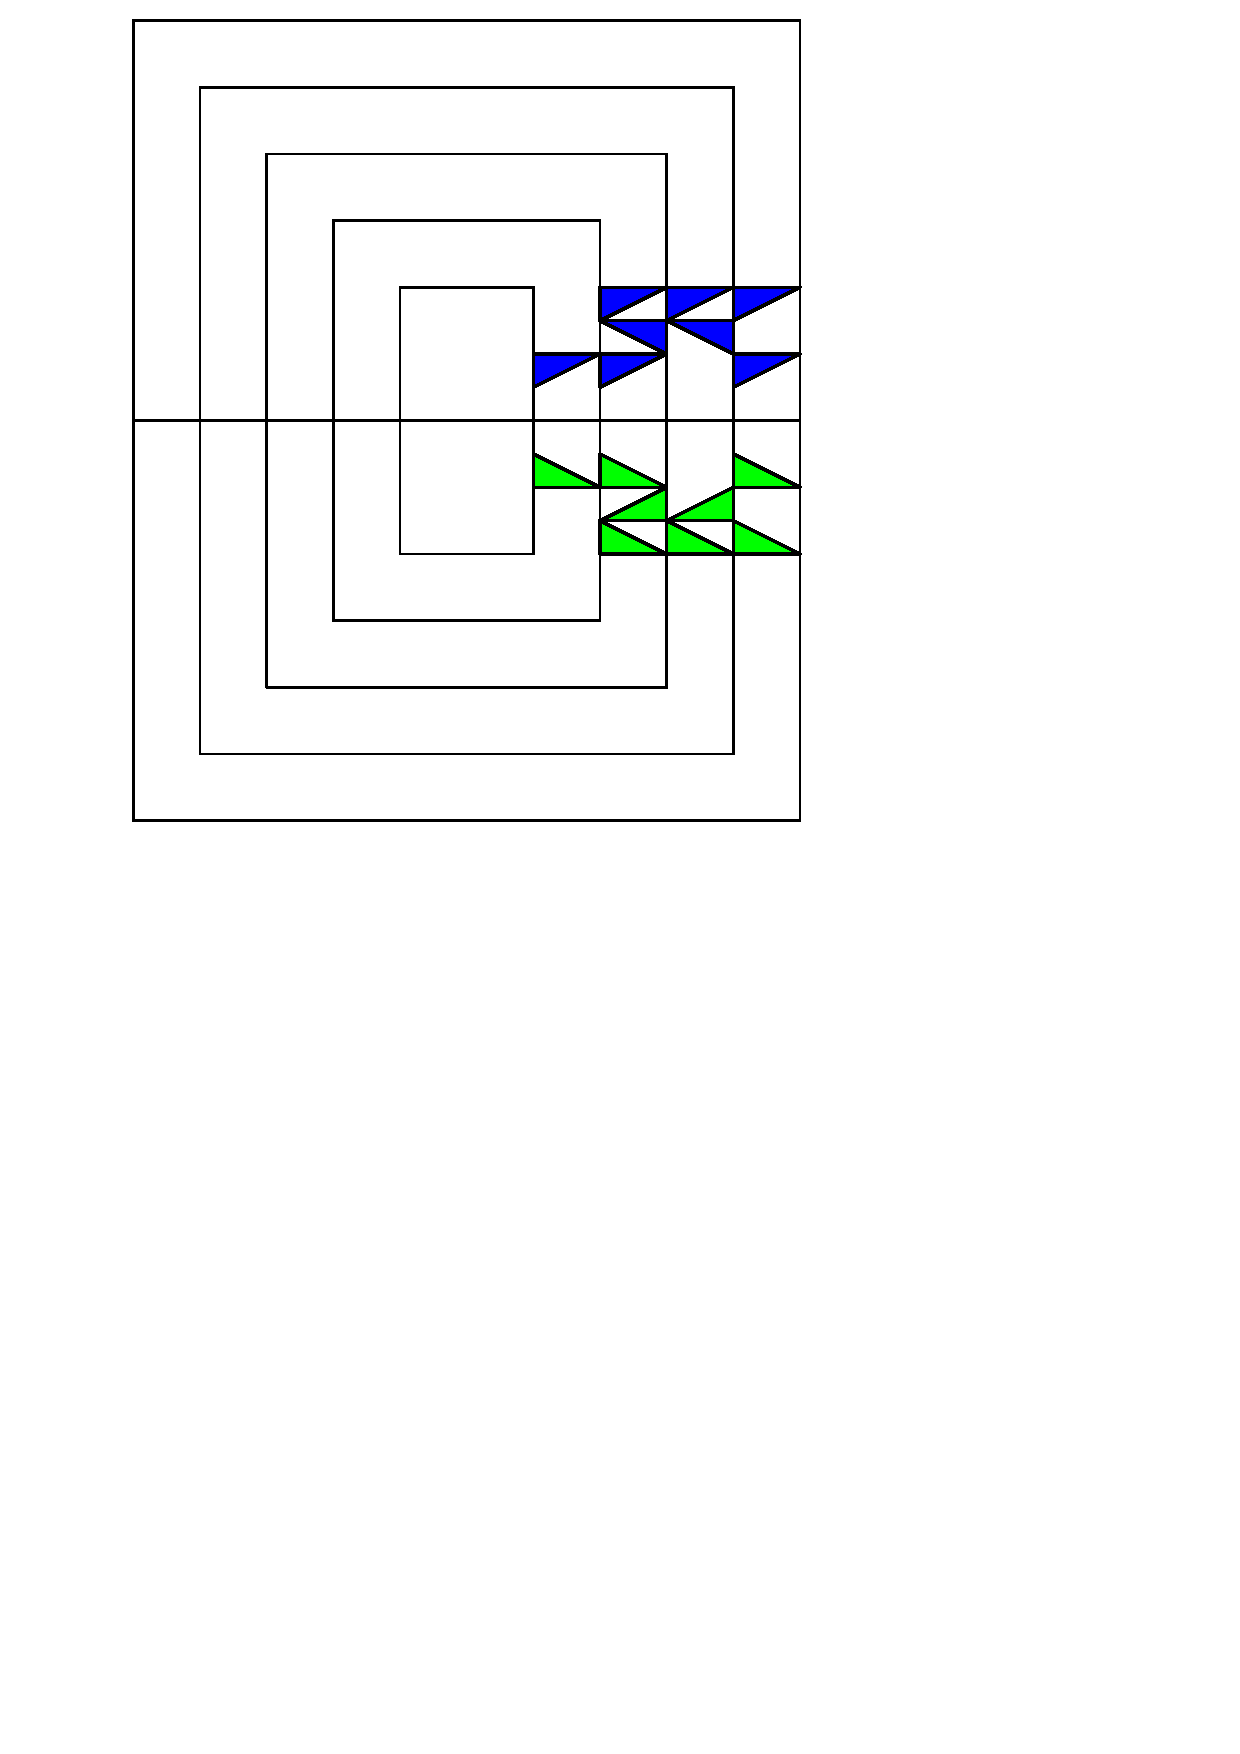
\includegraphics[scale=1]{graphics/logicengine.pdf}
\caption{A logic engine example.}\label{fig:logicengine-1}
\end{center}
\end{figure}
%Universality component
%\section{Logic Engine}
\section{Not All Equal 3 SAT Problem}
\begin{prob}[Not All Equal 3 SAT Problem]\label{prob:Satisfiability-2}%Problem/Question
Give a set of clauses $C$, each containing three boolean variables, can each clause contain at
least one true variable and one false variable?
\end{prob}
\subsection{The Logic Engine}
The logic engine simulates the well known Not All Equal 3 SAT Problem (NAE3SAT).
%add figure of logic engine.
\subsection{Construction of the Logic Engine}
The components of the logic engine are as follows: the rigid frame, the shaft, the armatures,
the chains, and the flags.  The \textit{rigid frame} is a rectangular enclosure with a horizontal
shaft place at mid-height.  The \textit{armatures} are concentric rectangular frames contained
within the rigid frame.  Each armature can rotate about the shaft; other motions on the armature
are disallowed.  Given an NAE3SAT, for each variable there is a corresponding armature. On each
armature, there are chains.  A pair of \textit{chains}, $a_j$ and $\bar{a}_j$ correspond to the
variable $x_j$ and $\bar{x}_j$ respectively.  The pair is placed on each armature, reflected at a
height of $h$ above and below the shaft, i.e. one place above the shave at a height of $h$, the
other placed below the shaft at a height of $-h$.
%insert an armature graphic

\subsection{Encoding the Logic Engine}
For each clause of an NAE3SAT, there exists a set of corresponding chains, namely the $h^\text{th}$
clause is the set of chains on the armatures at the $h^\text{th}$ row above and below the shaft. A
chain is \textit{flagged} if the corresponding variable resides within the clause.  The flag can
point in either the left or right directions indicating a truth assignment for that variable within
the clause.  A flag is attached to the $i^\text{th}$ chain of every $a_j^\text{th}$ and
$\bar{a}_j^\text{th}$ chain with the following exceptions:
\begin{enumerate}
 \item if the variable $x_j$  is in clause $C_i$, then link $i$ of $a_j$ is unflagged,
 \item if the variable $\bar{x}_j$ is in clause $C_i$, then link $i$ of $a_j$ is unflagged.
\end{enumerate}
\begin{thm}\label{thm:Satisfiability-1}
 An instance of $NAE3SAT$ is a ``yes'' instance if and only if the corresponding logic engine has a
flat, collision-free configuration.
\end{thm}
\begin{pf}
 If an instance of $NAE3SAT$ is a ``yes'', then every clause in $C$ contains at least one true
variable and one false variable.  Now suppose the following truth assignment:
\begin{equation}\label{eqn:Satisfiability-1}
                                                                                                                                    52,1          75%

